\documentclass{beamer}
\usepackage[utf8]{inputenc}
\usepackage{minted}
\usepackage{amsmath}
\usepackage{fancyvrb}
\usepackage{xspace}


\newcommand{\email}[1]{\href{mailto:#1}{\texttt{#1}}}

\title[petsc4py]{PETSc for Python}
\subtitle[]{\href{http://petsc4py.googlecode.com}%
           {\texttt{http://petsc4py.googlecode.com}}}
\author[L.~Dalcin\inst{1} \and K.~Kees\inst{2}]%
{
  Lisandro~Dalcin\inst{1} \and ~~~~~Christopher~Kees\inst{2}\\ 
  \email{dalcinl@gmail.com} \and \email{cekees@gmail.com}
}
\institute[CONICET/ERDC]
{
  \inst{1}%
  Centro Internacional de Métodos Computacionales en Ingeniería\\
  Consejo Nacional de Investigaciones Científicas y Técnicas\\
  Santa Fe, Argentina
  \and
  \inst{2}%
  Coastal and Hydraulics Laboratory\\
  US Army Engineer Research and Development Center\\
  Vicksburg, MS
}
\date [CSE '11]
{
  SIAM CSE 2011\\
  February 28 -- March 4, 2011\\
  Reno, Nevada
}

\AtBeginSection[]
{
  \begin{frame}
    \tableofcontents[currentsection]
  \end{frame}
}

\newcommand{\Cpp}{C\protect\raisebox{.18ex}{++}\xspace}

\begin{document}
\begin{frame}
  \titlepage
\end{frame}

\section*{Outline}
\begin{frame}
  \frametitle{Outline}
  \tableofcontents
\end{frame}

% --- Overview ---

\section{Overview}

\begin{frame}
  \frametitle{What is \textbf{petsc4py}?}  

  Python bindings for \textbf{PETSc}, the \emph{Portable Extensible
    Toolkit for Scientific Computation}.  
  
  \bigskip
 
  A \emph{good friend} of \textbf{petsc4py} is:
  \begin{itemize}
  \item \textbf{mpi4py}: Python bindings for \textbf{MPI}, the
    \emph{Message Passing Interface}.
  \end{itemize}
  \medskip
  Other two projects depend on petsc4py:
  \begin{itemize}
  \item \textbf{slepc4py}: Python bindings for \textbf{SLEPc}, the
    \emph{Scalable Library for Eigenvalue Problem Computations}.
  \item \textbf{tao4py}: Python bindings for \textbf{TAO}, the
    \emph{Toolkit for Advanced Optimization}.
  \end{itemize}
\end{frame}

\begin{frame}
  \frametitle{Implementation}
  Implemented with Cython \url{http://www.cython.org}
  \begin{itemize}
  \item Code base far easier to write, maintain, and extend.
  \item Faster than other solutions (mixed Python and C codes).
  \item Easier to cross language boundaries (reuse C/\Cpp/Fortran).
  \end{itemize}
\end{frame}

\begin{frame}
  \frametitle{Implementation - Cython [1]}
  \small\inputminted[firstline=1]{cython}{cython.pxi}
\end{frame}
\begin{frame}
  \frametitle{Implementation - Cython [2]}
  \small\inputminted[firstline=3]{cython}{cython.pyx}
\end{frame}

\begin{frame}
  \frametitle{Features -- PETSc components}
  \begin{itemize}
  \item \textbf{Index Sets}: permutations, indexing into vectors, renumbering.
  \item \textbf{Vectors}: sequential and distributed.
  \item \textbf{Matrices}: sequential and distributed, sparse and dense.
  \item \textbf{Distributed Arrays}: regular grid-based problems.
  \item \textbf{Linear Solvers}: Krylov subspace methods.
  \item \textbf{Preconditioners}: sparse direct solvers, multigrid
  \item \textbf{Nonlinear Solvers}: line search, trust region, matrix-free.
  \item \textbf{Timesteppers}: time-dependent, linear and nonlinear PDE's.
  \end{itemize}
\end{frame}

\begin{frame}
  \frametitle{Features -- Interoperability}
  Support for wrapping other PETSc-based codes.
  \begin{itemize}
  \item You can use \textbf{SWIG} (\textsl{typemaps} provided).
  \item You can use \textbf{F2Py} (\texttt{fortran} attribute).
  \end{itemize}
\end{frame}

\begin{frame}[fragile]
  \frametitle{Features -- Easy installation}
\begin{minted}{sh}
$ virtualenv --no-site-packages ENV
$ source ENV/bin/activate

(ENV) $ pip install slepc4py
Downloading/unpacking slepc4py
Downloading/unpacking petsc4py (from slepc4py)
Downloading/unpacking slepc (from slepc4py)
Downloading/unpacking petsc (from petsc4py->slepc4py)
Downloading/unpacking numpy (from petsc4py->slepc4py)
Installing collected packages: numpy, petsc, petsc4py,
                               slepc, slepc4py
(ENV) $
\end{minted}
\end{frame}

% --- Vectors & Matrices---

\section{Vectors \& Matrices}

\begin{frame}
  \frametitle{Vectors (\texttt{Vec}) -- Conjugate Gradients Method}
  \begin{columns}[t]
    \begin{column}{.45\textwidth}
      \tiny
      \begin{equation*}
        \begin{split}
          & cg(A,x,b,i_{max},\epsilon): \\
          & \quad i \Leftarrow 0 \\
          & \quad r \Leftarrow b - A x \\
          & \quad d \Leftarrow r \\
          & \quad \delta_{0} \Leftarrow r^T r \\
          & \quad \delta_{   } \Leftarrow \delta_{0} \\
          & \quad \text{while}\;\; i < i_{max} \text{ and } \\
          & \quad\quad\qquad  \delta_{   } > \delta_{0} \epsilon^2 \text{ do} :\\
          & \quad\quad\quad  q \Leftarrow Ad \\
          & \quad\quad\quad  \alpha \Leftarrow \frac{\delta_{   }}{d^T q} \\
          & \quad\quad\quad  x \Leftarrow x + \alpha d\\
          & \quad\quad\quad  r \Leftarrow r - \alpha q\\
          & \quad\quad\quad  \delta_{old} \Leftarrow \delta_{   } \\
          & \quad\quad\quad  \delta_{   } \Leftarrow r^T r \\
          & \quad\quad\quad  \beta \Leftarrow \frac{\delta_{   }}{\delta_{old}} \\
          & \quad\quad\quad  d \Leftarrow r + \beta d\\
          & \quad\quad\quad  i \Leftarrow i + 1
        \end{split}
      \end{equation*}
    \end{column}
    \begin{column}{.45\textwidth}
      \tiny\inputminted[linenos]{python}{petsc4py_vec.py}
    \end{column}
  \end{columns}
\end{frame}

\begin{frame}
  \frametitle{Matrices (\texttt{Mat}) [1]}
  \small\inputminted[linenos]{python}{petsc4py_mat_1.py}
\end{frame}

\begin{frame}
  \frametitle{Matrices (\texttt{Mat}) [2]}
  \small\inputminted[linenos]{python}{petsc4py_mat_2.py}
\end{frame}

% --- Linear Solvers  ---

\section{Linear Solvers}

\begin{frame}
  \frametitle{Linear Solvers (\texttt{KSP+PC})}
  \small\inputminted[linenos]{python}{petsc4py_ksp.py}
\end{frame}

% --- Nonlinear Solvers  ---

\section{Nonlinear Solvers}

\begin{frame}
  \frametitle{Nonlinear Solvers (\texttt{SNES}) [1]}
  \scriptsize\inputminted[linenos]{python}{petsc4py_snes_1.py}
\end{frame}

\begin{frame}
  \frametitle{Nonlinear Solvers (\texttt{SNES}) [2]}
  \small\inputminted[linenos]{python}{petsc4py_snes_2.py}
\end{frame}

% --- Interoperability ---

\section{Interoperability}

\begin{frame}
  \frametitle{Interoperability -- \textbf{SWIG}}
  \small
  \inputminted[linenos]{c}{wrap_swig.i}
\end{frame}

\begin{frame}
  \frametitle{Interoperability -- \textbf{F2Py}}
  \scriptsize
  \inputminted[linenos]{fortran}{wrap_f2py.pyf}
\end{frame}

% --- Performance ---

\section{Performance}

\newcommand{\onehalf}{\frac{1}{2}}
\newcommand{\pder}[2]{\ensuremath{\frac{\partial#1}{\partial#2}}}

\begin{frame}
  \frametitle{Performance}
  Consider the following diffusive, unsteady, non-linear, scalar
  problem in the unit cube $\Omega=(x,y,z)=(0,1)^3$
  \begin{itemize}
  \item PDE, boundary and initial conditions:
    \begin{equation}
      \begin{aligned}
        \pder{\phi}{t}-\nabla \cdot \left(\kappa(\phi)\nabla \phi \right) &= G
        ~~~\text{on $\Omega \times (0,T]$}\\
        \pder{\phi}{\mathbf{n}} &= 0 
        ~~~\text{at $\partial\Omega \times [0,T]$}\\
        \phi &= \phi^0
        ~~~\text{at $t=0$},
      \end{aligned}
    \end{equation}
  \item Nonlinear diffusion and line source terms:
    \begin{equation} 
      \begin{aligned}
        \kappa(\phi)=
        \begin{cases}
          1 ~~~&\text{if } \phi \ge 0 \\
          \frac{1}{1+\phi^2} ~~~&\text{if } \phi < 0
        \end{cases}\\
        G(x=\dfrac{1}{4},y=\frac{1}{4},\frac{1}{2}<z<1) = -300
      \end{aligned}
    \end{equation}
  \end{itemize}
\end{frame}

\begin{frame}
  \frametitle{Performance --Discretization}
\begin{itemize}
\item finite differences in space
\item backward Euler in time
\end{itemize}
\vfill
\begin{equation}
  \frac{1}{\Delta t}(\phi^{n+1}_{i,j,k}-\phi^{n}_{i,j,k}) - 
  L_{i,j,k}(\kappa,\phi^{n+1}) - G_{i,j,k} = 0 
\end{equation}
\begin{equation}
\footnotesize
\begin{split}
    L_{i,j,k}(\kappa,\phi) = %\\
     &\frac{\kappa[i-\onehalf]}{(\Delta x_1)^2}                \phi[i-1]%
     -\frac{\kappa[i-\onehalf]+\kappa[i+\onehalf]}{(\Delta x_1)^2} \phi[0]%
     +\frac{\kappa[i+\onehalf]}{(\Delta x_1)^2}               \phi[i+1] +\\
    +&\frac{\kappa[j-\onehalf]}{(\Delta x_2)^2}               \phi[j-1]%
     -\frac{\kappa[j-\onehalf]+\kappa[j+\onehalf]}{(\Delta x_2)^2} \phi[0]%
     +\frac{\kappa[j+\onehalf]}{(\Delta x_2)^2}               \phi[j+1] +\\
    +&\frac{\kappa[k-\onehalf]}{(\Delta x_3)^2}               \phi[k-1]%
     -\frac{\kappa[k-\onehalf]+\kappa[k+\onehalf]}{(\Delta x_3)^2} \phi[0]%
     +\frac{\kappa[k+\onehalf]}{(\Delta x_3)^2}               \phi[k+1]
\end{split}
\end{equation}
(notation: %
$[0]=(i,j,k)$, $[i\pm\frac{1}{2}]=(i\pm\frac{1}{2},j,k)$, %
and so on)
\end{frame}

\begin{frame}
  \frametitle{Performance -- Python+F90 versus C+F90}
  Basically a measure of Python calling overhead \ldots
  \begin{itemize}
  \item equivalent Python and C codes for the drivers
  \item common Fortran 90 code for the nonlinear residual
  \item use matrix--free for the nonlinear problems
  \end{itemize}
  \begin{center}
    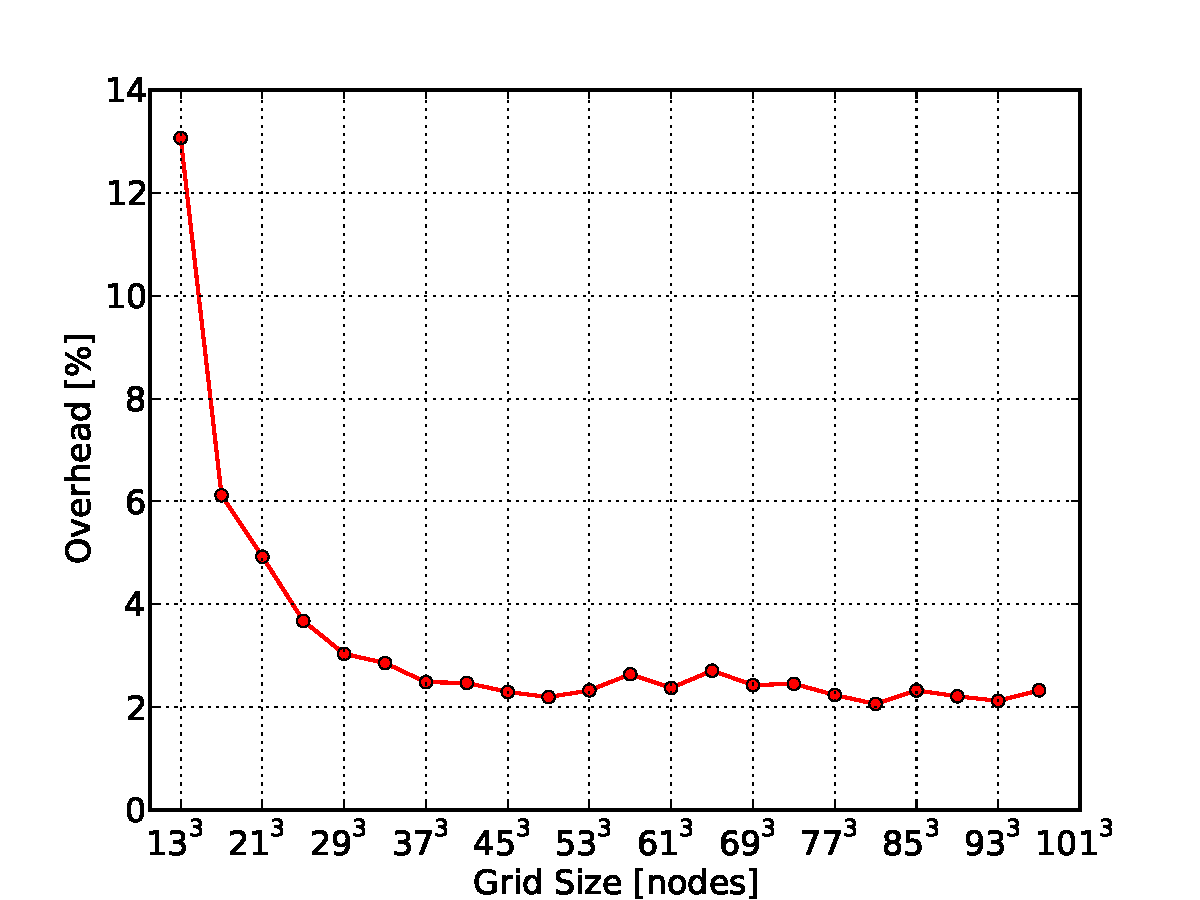
\includegraphics[scale=0.4]{petsc4py_oh.pdf}
  \end{center}
\end{frame}


% --- Closing ---

\section*{Closing}

\begin{frame}
  \Large
  Do not hesitate to ask for help \ldots 
  \bigskip
  \begin{itemize}
  \item Mailing List: \email{petsc-users@mcs.anl.gov}
  \item Mail\&Chat:   \email{dalcinl@gmail.com}
  \item Project Page: \url{http://petsc4py.googlecode.com}
  \end{itemize}
  \bigskip
  \begin{centering}
    \Huge Thanks!\par
  \end{centering}
\end{frame}

\end{document}


% Local Variables:
% mode: latex
% TeX-PDF-mode: t
% End:
